\documentclass{article}
\usepackage{../fasy-hw}

%% UPDATE these variables:
\renewcommand{\hwnum}{3}
\title{Discrete Structures, Homework \hwnum}
\author{Robert Marsh, JamesBean}
\collab{n/a}
\date{due: 19 February 2021}

\begin{document}

\maketitle

This homework assignment should be
submitted as a single PDF file both to D2L and to Gradescope.

General homework expectations:
\begin{itemize}
    \item Homework should be typeset using LaTex.
    \item Answers should be in complete sentences and proofread.
    \item You will not plagiarize.  \item List collaborators at the start of each question using the \texttt{collab} command.
    \item Put your answers where the \texttt{todo} command currently is (and
        remove the \texttt{todo}, but not the word \texttt{Answer}).
\end{itemize}

% ============================================
% ============================================
\collab{n/a} \nextprob{Negations}
% ============================================
% ============================================
Negate the following statements:

\begin{enumerate}

    \item Each ``Clean 'Cat Kit''  contains a cloth mask and a refillable hand
        sanitizer.

        \paragraph{Answer}
        There exists a ``Clean `Cat Kit`` that does not contain a cloth mask or does not contain a refillable hand sanitizer.

    \item There exists a boat docked in New Jersey that I have steered.

        \paragraph{Answer}
        Each boat docked in New Jersey is one that I have steered.

    \item There exists an island in the Ohio River with a bowling alley and a
        university track field.

        \paragraph{Answer}
        Each island in the Ohio River does not have a bowling alley or does not have a university track field.

    \item Both my sister and I can climb every route at Spire.

        \paragraph{Answer}
        There exist a route at Spire that my sister can't climb or I can't climb.

\end{enumerate}

% ============================================
% ============================================
\collab{n/a} \nextprob{Definitions}
% ============================================
% ============================================
Use the definitions provided in the course textbook to prove that every prime
number except~$2$ is odd.

\paragraph{Answer}

\begin{itemize}
\item To be proved: every prime number $n$ (except 2) is odd.
\item By the definition of even, $\forall$ even integers $n$ $\exists$ integer $k$ such that $n = 2 * k$
\item Through algebra, $k = \frac{n}{2}$
\item Next, by the definition of prime, $n$ is prime $\Leftrightarrow$  $\forall$ positive integers $r$ and $s$, if $n = rs$ then either $r=1$ and $s=n$ or $r=n$ and $s=1$
\item Let $r=2$ and $s=k$ 
\item By substitution, $n = 2 * \frac{n}{2}$
\item Because $\exists$ positive integers $r$ and $s$ where $n = rs$ and either $r \neq 1$ or $s \neq n$ and $r \neq n$ or $s \neq 1$, $n$ is not prime when $n \neq 2$
\item Hence, all even numbers that are not 2 are not prime numbers
\item Hence, all prime numbers that are not 2 are not even (Modus Tollens)
\item Any Integer is either even or odd, by Theorem 4.4.2 'The Parity Property'
\item Because all prime numbers that are not 2 are not even, all prime numbers that are not 2 are odd. [\it{This is what was to be shown.}]
\end{itemize}
%
% ============================================
% ============================================
\collab{\todo{}}
\nextprob{Four Colors Suffice}
% ============================================
% ============================================
Read Chapters $2$ and $3$ of \emph{Four Colors Suffice} and answer the following questions:

\begin{enumerate}

    \item Who are the Austrian(s) mentioned in Chapters $1$--$3$, and what was their
        contribution mentioned in the book?

        \paragraph{Answer}
        \todo{your answer here.}

    \item Write a statement of the four color theorem using a universal
        quantifier.

        \paragraph{Answer}
        For each map $m$, if it meets the prerequisites of the four-color theorem, then it may be colored with only 4 different colors where no two neighboring vertices ("regions/countries") are the same color.

    \item What is the definition of a $k$-coloring of a graph?

        \paragraph{Answer}
        A $k$-colored graph is a graph which has each vertex colored from a set of $k$ colors, with no adjacent vertexes of the same color.

    \item Prove or disprove: all plane graphs (maps) are three-colorable.

        \paragraph{Answer}
        \begin{figure}[h]
            \centering
            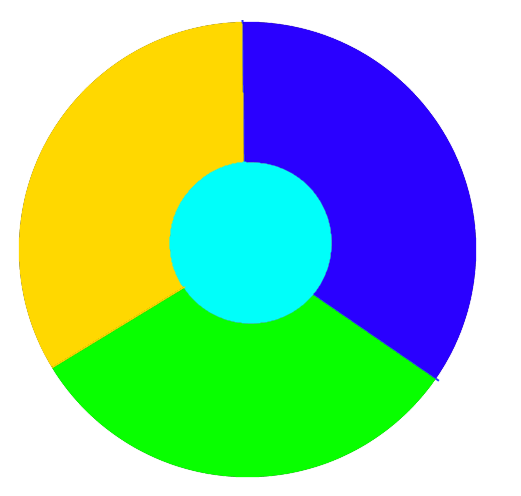
\includegraphics[width=3.5in]{3map}
            \caption{A Plane Graph That is Not Three-Colorable}\label{fig:4-color map}
        \end{figure}

    \begin{itemize}
        \item For each plane graph $m$, $m$ is three-colorable.
        \item Because each region of this map is touching 3 other regions, it is not three colorable.
        \item Hence, not all plane graphs are three-colorable.
    \end{itemize}

    \item Assuming the four color theorem holds, prove or disprove: six colors
        suffice to color a plane graph.

        \paragraph{Answer}
        By definition of the four color theorem, four colors suffice to color a plane graph. After color a plane graph with 4 colors, we can change the color of two vertex to make it into a six color graph. Therefore, six colors suffice as well.

    \item Give an example of a map with at least five faces that has a
        two-coloring.  Be sure to provide a coloring as evidence that the map is
        two-colorable.

        \paragraph{Answer}
        A chess board.

    \item Euler's formula states that if we have a map on the sphere or plane
        and count the exterior face as a face, then F-E+V=2.  Does this equation
        hold if the map is drawn on a M\"obius band? Why or why not? (Note:
        here, the boundary of the M\"obius band must be represented in the graph
        defining the map, and no ``country'' can be on the same side of a single
        edge.)

        \paragraph{Answer}
        \todo{your answer here.}

    \item In your own words, explain the joke: ``A topologist cannot tell the
        difference between a coffee cup and a donut.''  You are encouraged to
        use Wikipedia to formulate your answer, but be sure to cite sources.

        \paragraph{Answer}
        A coffee cup and a donut both are a mass with one hole, and can be reshaped to form one another without breaking this property. Topologists do not care about the exact shape of the object, so long as it maintains this one-hole property.

\end{enumerate}

% ============================================
% ============================================
\collab{https://www.britannica.com/biography/Ada-Lovelace}
\nextprob{Ada Lovelace}
% ============================================
% ============================================

Write a short (1-2 paragraph) biography of Ada Lovelace.
\textbf{In your own words}, describe who they are and why they are important in
the history of computer science.  If you use external resources, please provide
proper citations (see the `hw/bib-ex` folder for examples of how to use
citations). If you do not use external sources, please write ``I did not
use any sources to write this biography'' as the last sentence of the
biography.

\paragraph{Answer}

Ada Lovelace was a woman that lived during the 19th century, studying mathematics independently from tutors such as University of London professors. The focus of her notoriety revolves around her work with Charles Babbage on the machine known as the "Charles Babbage Analytical Machine". Her primary published paper was a translation from an Italian mathematician, Luigi Federico Menebrea, of Luigi's notes on the machine. In translating this to English, Lovelace wrote an additional set of notes elaborating on the machine and possible further uses. Although the machine was barely built and these concepts never were produced, these theories provide a foundation for the set of computational instructions that we used in computer science today.

% %% ... the bibliography
% \newpage
% \bibliographystyle{acm}
% \bibliography{biblio}

\end{document}

